% $Id$
%
%           Copyright © 2006 by ACcESS MNRF
%               http://www.access.edu.au
%         Primary Business: Queensland, Australia.
%   Licensed under the Open Software License version 3.0
%      http://www.opensource.org/licenses/osl-3.0.php
%


\chapter{The module \escript}
\label{ESCRIPT CHAP}


\begin{figure}
\includegraphics[width=\textwidth]{figures/EscriptDiagram1.eps}
\caption{\label{ESCRIPT DEP}Dependency of Function Spaces. An arrow indicates that a function in the 
function space at the starting point can be interpreted as a function in the function space of the arrow target.}
\end{figure}

\escript is an extension of Python to handle functions represented by their values on
\DataSamplePoints for the geometrical region on which
the function is defined. The region as well as the method which is used 
to interpolate value on the \DataSamplePoints is defined by     
\Domain class objects. For instance when using 
the finite element method (FEM) \index{finite element method} 
\Domain object holds the information about the FEM mesh, eg. 
a table of nodes and a table of elements. Although \Domain contains
the discretization method to be used \escript does not use this information directly.
\Domain objects are created from a module which want to make use 
\escript, e.g. \finley.

The solution of a PDE is a function of its location in the domain of interest $\Omega$. 
When solving a partial differential equation \index{partial differential equation} (PDE) using FEM
the solution is (piecewise) differentiable but, in general, its gradient
is discontinuous. To reflect these different degrees of smoothness different
representations of the functions are used. For instance; in FEM
the displacement field is represented by its values at the nodes of the mesh, while the 
strain, which is the symmetric part of the gradient of the displacement field, is stored on the 
element centers. To be able to classify functions with respect to their smoothness, \escript has the
concept of the "function space". A function space is described by a \FunctionSpace object.
The following statement generates the object \var{solution_space} which is 
a \FunctionSpace object and provides access to the function space of 
PDE solutions on the \Domain \var{mydomain}:
\begin{python}
solution_space=Solution(mydomain)
\end{python}
The following generators for function spaces on a \Domain \var{mydomain} are available: 
\begin{itemize}
\item \var{Solution(mydomain)}: solutions of a PDE.
\item \var{ReducedSolution(mydomain)}: solutions of a PDE with a reduced smoothness requirement.  
\item \var{ContinuousFunction(mydomain)}: continuous functions, eg. a temperature distribution.
\item \var{Function(mydomain)}: general functions which are not necessarily continuous, eg. a stress field.
\item \var{FunctionOnBoundary(mydomain)}: functions on the boundary of the domain, eg. a surface pressure.
\item \var{FunctionOnContact0(mydomain)}: functions on side $0$ of the discontinuity. 
\item \var{FunctionOnContact1(mydomain)}: functions on side $1$ of the discontinuity.
\end{itemize}
The reduced smoothness for PDE solution is often used to fulfill the Ladyzhenskaya–-Babuska–-Brezzi condition \cite{LBB} when 
solving saddle point problems \index{saddle point problems}, eg. the Stokes equation.
A discontinuity \index{discontinuity} is a region within the domain across which functions may be discontinuous.  
The location of discontinuity is defined in the \Domain object.
\fig{ESCRIPT DEP} shows the dependency between the types of function spaces. 
The solution of a PDE is a continuous function. Any continuous function can be seen as a general function
on the domain and can be restricted to the boundary as well as to any side of the 
discontinuity (the result will be different depending on 
which side is chosen). Functions on any side of the  
discontinuity can be seen as a function on the corresponding other side. 
A function on the boundary or on one side of
the discontinuity cannot be seen as a general function on the domain as there are no values 
defined for the interior. For most PDE solver libraries
the space of the solution and continuous functions is identical, however in some cases, eg.
when periodic boundary conditions are used in \finley, a solution 
fulfils periodic boundary conditions while a continuous function does not have to be periodic.
   
The concept of function spaces describes the properties of 
functions and allows abstraction from the actual representation 
of the function in the context of a particular application. For instance, 
in the FEM context a
function in the \Function function space
is typically represented by its values at the element center, 
but in a finite difference scheme the edge midpoint of cells is preferred. 
Using the concept of function spaces 
allows the user to run the same script on different
PDE solver libraries by just changing the creator of the \Domain object.     
Changing the function space of a particular function
will typically lead to a change of its representation. 
So, when seen as a general function,
a continuous function which is typically represented by its values
on the node of the FEM mesh or finite difference grid 
must be interpolated to the element centers or the cell edges,
respectively.

\Data class objects store functions of the location in a domain. 
The function is represented through its values on \DataSamplePoints where
the \DataSamplePoints are chosen according to the function space 
of the function.  
\Data class objects are used to define the coefficients
of the PDEs to be solved by a PDE solver library 
and to store the returned solutions.

The values of the function have a rank which gives the
number of indices, and a \Shape defining the range of each index.
The rank in \escript is limited to the range $0$ through $4$ and
it is assumed that the rank and \Shape is the same for all \DataSamplePoints.
The \Shape of a \Data object is a tuple \var{s} of integers. The length
of \var{s} is the rank of the \Data object and \var{s[i]} is the maximum
value for the \var{i}-th index.
For instance, a stress field has rank $2$ and 
\Shape $(d,d)$ where $d$ is the spatial dimension.
The following statement creates the \Data object
\var{mydat} representing a 
continuous function with values 
of \Shape $(2,3)$ and rank $2$:
\begin{python}
mydat=Data(value=1,what=ContinuousFunction(myDomain),shape=(2,3))
\end{python}
The initial value is the constant $1$ for all \DataSamplePoints and
all components.

\Data objects can also be created from any \numarray
array or any object, such as a list of floating point numbers, 
that can be converted into a \numarray.NumArray \Ref{NUMARRAY}. 
The following two statements
create objects which are equivalent to \var{mydat}:
\begin{python}
mydat1=Data(value=numarray.ones((2,3)),what=ContinuousFunction(myDomain))
mydat2=Data(value=[[1,1],[1,1],[1,1]],what=ContinuousFunction(myDomain))
\end{python}
In the first case the initial value is \var{numarray.ones((2,3))}
which generates a $2 \times 3$ matrix as a \numarray.NumArray 
filled with ones. The \Shape of the created \Data object
it taken from the \Shape of the array. In the second
case, the creator converts the initial value, which is a list of lists,
and converts it into a \numarray.NumArray before creating the actual
\Data object.      

For convenience \escript provides creators for the most common types
of \Data objects in the following forms (\var{d} defines the 
spatial dimension):
\begin{itemize}
\item \var{Scalar(0,Function(mydomain))} is the same as \var{Data(0,Function(myDomain),(,))}, 
e.g a temperature field. 
\item \var{Vector(0,Function(mydomain))}is the same as \var{Data(0,Function(myDomain),(d))}, e.g
a velocity field.   
\item \var{Tensor(0,Function(mydomain))} is the same as \var{Data(0,Function(myDomain),(d,d))},
eg. a stress field.  
\item \var{Tensor4(0,Function(mydomain))} is the same as \var{Data(0,Function(myDomain),(d,d,d,d))}
eg. a Hook tensor field.   
\end{itemize}
Here the initial value is $0$ but any object that can be converted into a \numarray.NumArray and whose \Shape
is consistent with \Shape of the \Data object to be created can be used as the initial value.

\Data objects can be manipulated by applying unitary operations (eg. cos, sin, log) 
and can be combined by applying binary operations (eg. +, - ,* , /). 
It is to be emphasized that \escript itself does not handle any spatial dependencies as 
it does not know how values are interpreted by the processing PDE solver library. 
However \escript invokes interpolation if this is needed during data manipulations. 
Typically, this occurs in binary operation when both arguments belong to different
function spaces or when data are handed over to a PDE solver library 
which requires functions to be represented in a particular way. 

The following example shows the usage of {\tt Data} objects: Assume we have a
displacement field $u$ and we want to calculate the corresponding stress field
$\sigma$ using the linear--elastic isotropic material model
\begin{eqnarray}\label{eq: linear elastic stress}
\sigma\hackscore {ij}=\lambda u\hackscore {k,k} \delta\hackscore {ij} + \mu ( u\hackscore {i,j} + u\hackscore {j,i})
\end{eqnarray}
where $\delta\hackscore {ij}$ is the Kronecker symbol and 
$\lambda$ and $\mu$ are the Lame coefficients. The following function
takes the displacement {\tt u} and the Lame coefficients
\var{lam} and \var{mu} as arguments and returns the corresponding stress:
\begin{python}
from esys.escript import *
def getStress(u,lam,mu):
  d=u.getDomain().getDim()
  g=grad(u)
  stress=lam*trace(g)*kronecker(d)+mu*(g+transpose(g))
  return stress     
\end{python}
The variable 
\var{d} gives the spatial dimension of the 
domain on which the displacements are defined.
\var{kronecker} returns the Kronecker symbol with indexes 
$i$ and $j$ running from $0$ to \var{d}-1. The call \var{grad(u)} requires 
the displacement field \var{u} to be in the \var{Solution} or \ContinuousFunction
function space. The result \var{g} as well as the returned stress will be in the \Function function space. 
If \var{u} is available, eg. by solving a PDE, \var{getStress} might be called
in the following way:
\begin{python}
s=getStress(u,1.,2.)
\end{python}
However \var{getStress} can also be called with \Data objects as values for
\var{lam} and \var{mu} which,
for instance in the case of a temperature dependency, are calculated by an expression. 
The following call is equivalent to the previous example:
\begin{python}
lam=Scalar(1.,ContinuousFunction(mydomain))
mu=Scalar(2.,Function(mydomain))
s=getStress(u,lam,mu)
\end{python}
The function \var{lam} belongs to the \ContinuousFunction function space
but with \var{g} the function \var{trace(g)} is in the \Function function space.
Therefore the evaluation of the product \var{lam*trace(g)} in the stress calculation 
produces a problem, as both functions are represented differently, eg. in FEM
\var{lam} by its values on the node, and in \var{trace(g)} by its values at the element centers.
In the case of inconsistent function spaces of arguments in a binary operation, \escript 
interprets the arguments in the appropriate function space according to the inclusion 
defined in Table~\ref{ESCRIPT DEP}. In this example that means
 \escript sees \var{lam} as a function of the \Function function space. 
In the context of FEM this means the nodal values of 
\var{lam} are interpolated to the element centers. Behind the scenes
\escript calls the appropriate function from the PDE solver library.

\begin{figure}
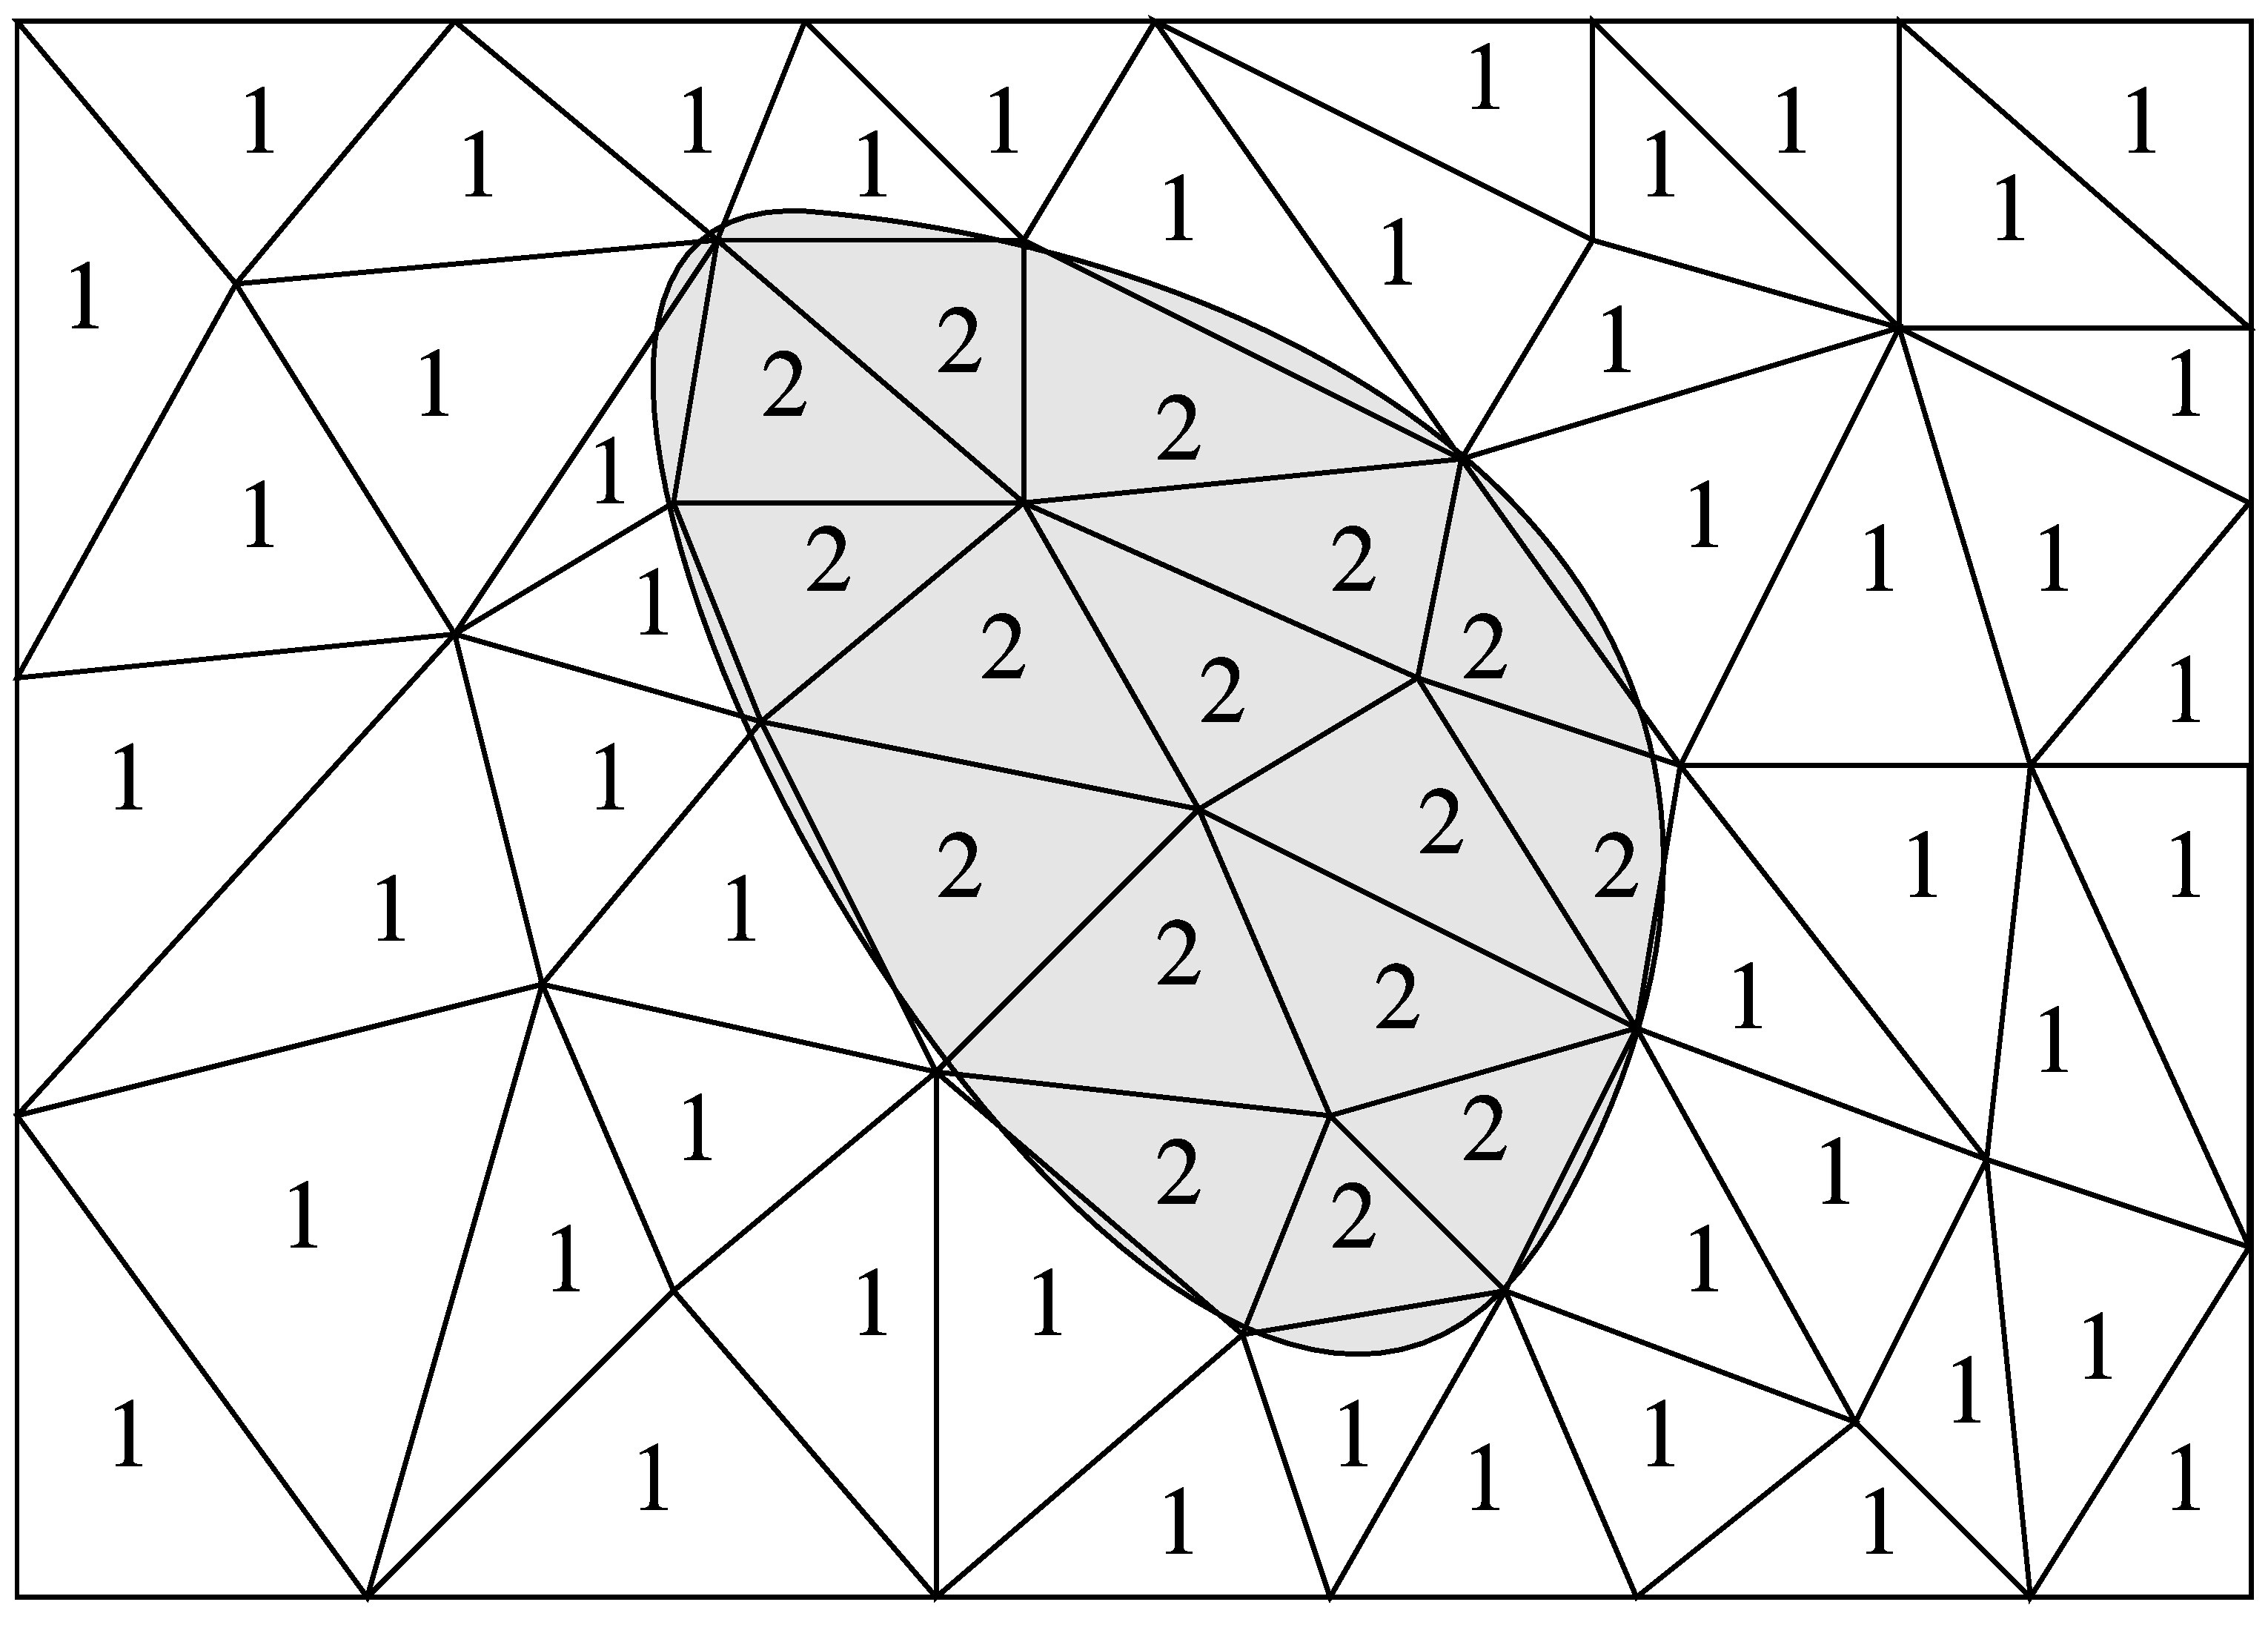
\includegraphics[width=\textwidth]{figures/EscriptDiagram2.eps}
\caption{\label{Figure: tag}Element Tagging. A rectangular mesh over a region with two rock types {\it white} and {\it gray}.
The number in each cell refers to the major rock type present in the cell ($1$ for {\it white} and $2$ for {\it gray}).
}
\end{figure}

Material parameters such as the Lame coefficients are typically dependent on rock types present in the 
area of interest. A common technique to handle these kinds of material parameters is "tagging". \fig{Figure: tag}
shows an example. In this case two rock types {\it white} and {\it gray} can be found in the domain. The domain
is subdivided into triangular shaped cells. Each 
cell has a tag indicating the rock type predominately found in this cell. Here $1$ is used to indicate
rock type {\it white} and $2$ for rock type {\it gray}. The tags are assigned at the time when the cells are generated
and stored in the \Domain class object. To allow easier usage of tags names can be used. These names are typically defined 
at the time when the geometry is generated. 

The following statements show how for the
example of \fig{Figure: tag} and the stress calculation discussed before tagged values are used for
\var{lam}:
\begin{python}
lam=Scalar(value=2.,what=Function(mydomain))
insertTaggedValue(lam,white=30.,gray=5000.)
s=getStress(u,lam,2.)
\end{python}
In this example \var{lam} is set to $30$ for those cells with tag {\it white} (=$1$) and to $5000.$ for those cells 
with tag {\it gray} (=$2$_. The initial value $2$ of \var{lam} is used as a default value for the case when a tag
is encountered which has not been linked with a value. Note that the \var{getStress} method
is called without modification. \escript resolves the tags when \var{lam*trace(g)} is calculated.

The \Data class provides a transparent interface to various data representations and the 
translations between them. As shown in the example of stress calculation, this allows the user to
develop and test algorithms for a simple case (for instance with the Lame coefficients as constants)
and then without further modifications of the program code to apply the algorithm in a
more complex application (for instance a definition of the Lame coefficients using tags). 
As described here, there are three ways in which \Data objects are represented internally, constant, 
tagged, and expanded (other representations will become available in later versions of \escript):
In the constant case, if the same value is used at each sample point a single value is stored to save memory and compute time. 
Any operation on this constant data will only be performed on the single value. 
In the expanded case, each sample point has an individual value, eg. the solution of a PDE,
and the values are stored as a complete array. The tagged case has already been discussed above.
 
Values are accessed through a sample reference number. Operations on expanded \Data
objects have to be performed for each sample point individually. If tagged values are used values are
held in a dictionary. Operations on tagged data require processing the set of tagged values only, rather than 
processing the value for each individual sample point. 
\escript allows use of constant, tagged and expanded data in a single expression.

The \var{dump} method provides a possibility to save \Data objects to a file, for instance to restart a simuation
or to save data for visualization. The file format uses \netCDF which commonly is using the file extension
{\tt nc}. For instance to save the coordinates of the data points of the \FunctionSpace
\ContinuousFunction to the file {\tt x.nc} one uses:
\begin{python}
x=ContinuousFunction(mydomain).getX()
x.dump("x.nc")
\end{python}
In order to keep the dump files small {\tt x.nc} does not contain a representation of the \Domain. It has to be saved using 
apropriated methods of \var{mydomain} to be loaded before \var{x}. Alternatively, the \Domain can be reconstructed. 
To recover the object \var{x} one uses
\begin{python}
x=load("x.nc", mydomain)
\end{python}
The \Data object represented by {\tt x.nc} is tight to a \FunctionSpace - in this case \ContinuousFunction - but not 
o a \Domain. That means that \Data objects that are constant or tagged can be recovered with any \Domain. If the \Data object
is expanded, the number of data points in the file and of the \Domain for the particular \FunctionSpace must match. 
Moreover, the ordering of the value is checked using the reference identifiers provided by 
\FunctionSpace on the \Domain. In some cases, data points will be reordered.


\section{\escript Classes}
\declaremodule{extension}{esys.escript} 
\modulesynopsis{Data manipulation}

\subsection{\Domain class}
\begin{classdesc}{Domain}{}
A \Domain object is used to describe a geometrical region together with 
a way of representing functions over this region.
The \Domain class provides an abstract access to the domain of \FunctionSpace and \Data objects. 
\Domain itself has no initialization but implementations of \Domain are 
instantiated by numerical libraries making use of \Data objects. 
\end{classdesc}
The following methds are available:
\begin{methoddesc}[Domain]{getDim}{}
returns the spatial dimension of the \Domain.
\end{methoddesc}

\begin{methoddesc}[Domain]{getX}{}
returns the locations in the \Domain. The \FunctionSpace of the returned
\Data object is chosen by the \Domain implementation. Typically it will be
in the \Function.
\end{methoddesc}

\begin{methoddesc}[Domain]{setX}{newX}
assigns a new location to the \Domain. \var{newX} has to have \Shape $(d,)$
where $d$ is the spatial dimension of the domain. Typically \var{newX} must be
in the \ContinuousFunction but the space actually to be used depends on the \Domain implementation.
\end{methoddesc}

\begin{methoddesc}[Domain]{getNormal}{}
returns the surface normals on the boundary of the \Domain as \Data object.
\end{methoddesc}

\begin{methoddesc}[Domain]{getSize}{}
returns the local sample size, e.g. the element diameter, as \Data object.
\end{methoddesc}

\begin{methoddesc}[Domain]{setTagMap}{tag_name, tag}
defines a mapping of the tag name  \var{tag_name} to the \var{tag}. 
\end{methoddesc}
\begin{methoddesc}[Domain]{getTag}{tag_name}
returns the tag associated with the tag name \var{tag_name}.
\end{methoddesc}
\begin{methoddesc}[Domain]{isValidTagName}{tag_name}
return \True if \var{tag_name} is a valid tag name.
\end{methoddesc}

\begin{methoddesc}[Domain]{__eq__}{arg}
returns \True of the \Domain \var{arg} describes the same domain. Otherwise
\False is returned.
\end{methoddesc}

\begin{methoddesc}[Domain]{__ne__}{arg}
returns \True of the \Domain \var{arg} does not describe the same domain. 
Otherwise \False is returned.
\end{methoddesc}

\begin{methoddesc}[Domain]{__str__}{g}
returns string represention of the \Domain.
\end{methoddesc}

\subsection{\FunctionSpace class}
\begin{classdesc}{FunctionSpace}{}
\FunctionSpace objects are used to define properties of \Data objects, such as continuity. \FunctionSpace objects
are instantiated by generator functions. \Data objects in particular \FunctionSpace are
represented by their values at \DataSamplePoints which are defined by the type and the \Domain of the
\FunctionSpace.
\end{classdesc}
The following methods are available:
\begin{methoddesc}[FunctionSpace]{getDim}{}
returns the spatial dimension of the \Domain of the \FunctionSpace.
\end{methoddesc}



\begin{methoddesc}[FunctionSpace]{getX}{}
returns the location of the \DataSamplePoints.
\end{methoddesc}

\begin{methoddesc}[FunctionSpace]{getNormal}{}
If the domain of functions in the \FunctionSpace 
is a hypermanifold (e.g. the boundary of a domain)
the method returns the outer normal at each of the 
\DataSamplePoints. Otherwise an exception is raised.
\end{methoddesc}

\begin{methoddesc}[FunctionSpace]{getSize}{}
returns a \Data objects measuring the spacing of the \DataSamplePoints.  
The size may be zero.
\end{methoddesc}

\begin{methoddesc}[FunctionSpace]{getDomain}{}
returns the \Domain of the \FunctionSpace.
\end{methoddesc}

\begin{methoddesc}[FunctionSpace]{setTags}{new_tag, mask}
assigns a new tag \var{new_tag} to all data sample 
where \var{mask} is positive for a least one data point. 
\var{mask} must be defined on the this \FunctionSpace.
Use the \var{setTagMap} to assign a tage name to \var{new_tag}.
\end{methoddesc}

\begin{methoddesc}[FunctionSpace]{__eq__}{arg}
returns \True of the \Domain \var{arg} describes the same domain. Otherwise
\False is returned.
\end{methoddesc}

\begin{methoddesc}[FunctionSpace]{__ne__}{arg}
returns \True of the \Domain \var{arg} describes the note same domain. 
Otherwise \False is returned.
\end{methoddesc}

\begin{methoddesc}[Domain]{__str__}{g}
returns string represention of the \Domain.
\end{methoddesc}

The following function provide generators for \FunctionSpace objects:
\begin{funcdesc}{Function}{domain}
returns the \Function on the \Domain \var{domain}. \Data objects in this type of \Function
are defined over the whole geometrical region defined by \var{domain}. 
\end{funcdesc}

\begin{funcdesc}{ContinuousFunction}{domain}
returns the \ContinuousFunction on the \Domain domain. \Data objects in this type of \Function
are defined over the whole geometrical region defined by \var{domain} and assumed to represent
a continuous function.
\end{funcdesc}

\begin{funcdesc}{FunctionOnBoundary}{domain}
returns the \ContinuousFunction on the \Domain domain. \Data objects in this type of \Function
are defined on the boundary of the geometrical region defined by \var{domain}. 
\end{funcdesc}

\begin{funcdesc}{FunctionOnContactZero}{domain}
returns the \FunctionOnContactZero the \Domain domain. \Data objects in this type of \Function
are defined on side 0 of a discontinutiy  within the geometrical region defined by \var{domain}.
The discontinutiy is defined when \var{domain} is instantiated.
\end{funcdesc}

\begin{funcdesc}{FunctionOnContactOne}{domain}
returns the \FunctionOnContactOne on the \Domain domain. 
\Data objects in this type of \Function
are defined on side 1 of a discontinutiy  within the geometrical region defined by \var{domain}.
The discontinutiy is defined when \var{domain} is instantiated.
\end{funcdesc}

\begin{funcdesc}{Solution}{domain}
returns the \SolutionFS on the \Domain domain. \Data objects in this type of \Function
are defined on geometrical region defined by \var{domain} and are solutions of
partial differential equations \index{partial differential equation}. 
\end{funcdesc}

\begin{funcdesc}{ReducedSolution}{domain}
returns the \ReducedSolutionFS on the \Domain domain. \Data objects in this type of \Function
are defined on geometrical region defined by \var{domain} and are solutions of
partial differential equations \index{partial differential equation} with a reduced smoothness 
for the solution approximation.
\end{funcdesc}

\subsection{\Data Class}
\label{SEC ESCRIPT DATA}

The following table shows binary and unitary operations that can be applied to
\Data objects:
\begin{tableii}{l|l}{textrm}{expression}{Description}
\lineii{+\var{arg0}} {just \var{arg} \index{+}}
\lineii{-\var{arg0}} {swapping the sign\index{-}}
\lineii{\var{arg0}+\var{arg1}} {adds \var{arg0} and \var{arg1} \index{+}}
\lineii{\var{arg0}*\var{arg1}} {multiplies \var{arg0} and \var{arg1} \index{*}}
\lineii{\var{arg0}-\var{arg1}} {difference \var{arg1} from\var{arg1} \index{-}}
\lineii{\var{arg0}/\var{arg1}} {ratio \var{arg0} by \var{arg1} \index{/}}
\lineii{\var{arg0}**\var{arg1}} {raises \var{arg0} to the power of \var{arg1} \index{**}}
\end{tableii}
At least one of the arguments \var{arg0} or \var{arg1} must be a
\Data object. One of the arguments may be an object that can be
converted into a \Data object. If \var{arg0} or \var{arg1} are
defined on different \FunctionSpace an attempt is made to embed \var{arg0}
into the \FunctionSpace of \var{arg1} or to embed \var{arg1} into
the \FunctionSpace of \var{arg0}. Boths arguments must have the same
\Shape or one of the arguments my be of rank 0. In the
latter case it is assumed that the particular argument is of the same
\Shape as the other argument but constant over all components.

The returned \Data object has the same \Shape and is defined on
the \DataSamplePoints as \var{arg0} or \var{arg1}.

The following table shows the update operations that can be applied to
\Data objects:
\begin{tableii}{l|l}{textrm}{expression}{Description}
\lineii{\var{arg0}+=\var{arg2}} {adds \var{arg0} to \var{arg2} \index{+}}
\lineii{\var{arg0}*=\var{arg2}} {multiplies \var{arg0} with \var{arg2} \index{*}}
\lineii{\var{arg0}-=\var{arg2}} {subtracts \var{arg2} from\var{arg2} \index{-}}
\lineii{\var{arg0}/=\var{arg2}} {divides \var{arg0} by \var{arg2} \index{/}}
\lineii{\var{arg0}**=\var{arg2}} {raises \var{arg0} by \var{arg2} \index{**}}
\end{tableii}
\var{arg0} must be a \Data object. \var{arg1} must be a
\Data object or an object that can be converted into a
\Data object. \var{arg1} must have the same \Shape like
\var{arg1} or has rank 0.  In the latter case it is
assumed that the values of \var{arg1} are constant for all
components. \var{arg1} must be defined in the same \FunctionSpace as
\var{arg0} or it must be possible to interpolate \var{arg1} onto the
\FunctionSpace of \var{arg1}.

The \Data class supports getting slices as well as assigning new values to components in an existing
\Data object. \index{slicing}
The following expression for getting (expression on the right hand side of the
equal sign) and setting slices (expression on the left hand side of the
equal sign) are valid:
\begin{tableiii}{l|ll}{textrm}{rank of \var{arg}}{slicing expression}{\Shape of returned and assigned object}
\lineiii{0}{ no slicing }                      {-}
\lineiii{1}{\var{arg[l0:u0]}}                   {(\var{u0}-\var{l0},)}
\lineiii{2}{\var{arg[l0:u0,l1:u1]}}             {(\var{u0}-\var{l0},\var{u1}-\var{l1})}
\lineiii{3}{\var{arg[l0:u0,l1:u1,l2:u2]} }      {(\var{u0}-\var{l0},\var{u1}-\var{l1},\var{u2}-\var{l2})}
\lineiii{4}{\var{arg[l0:u0,l1:u1,l2:u2,l3:u3]}} {(\var{u0}-\var{l0},\var{u1}-\var{l1},\var{u2}-\var{l2},\var{u3}-\var{l3})}
\end{tableiii}
where 
$0 \le \var{l0} \le \var{u0} \le \var{s[0]}$,
$0 \le \var{l1} \le \var{u1} \le \var{s[1]}$, 
$0 \le \var{l2} \le \var{u2} \le \var{s[2]}$, 
$0 \le \var{l3} \le \var{u3} \le \var{s[3]}$ and \var{s} the \Shape if \var{arg}. 
Any of the lower indexes \var{l0}, \var{l1}, \var{l2} and \var{l3} may not be present in which case 
$0$ is assumed. 
Any of the upper indexes \var{u0}, \var{u1}, \var{u2} and \var{u3} may not be present in which case 
\var{s} is assumed. The lower and upper index may be identical, in which case the column and the lower or upper
index may be dropped. In the returned or in the object assigned to a slice the corresponding component is dropped,
i.e. the rank is reduced by one in comparison to \var{arg}.
The following examples show slicing usage:  
\begin{python}
t=Data(1.,(4,4,6,6),Function(mydomain))
t[1,1,1,0]=9.
s=t[:2,:,2:6,5] # s has rank 3
s[:,:,1]=1.
t[:2,:2,5,5]=s[2:4,1,:2]
\end{python}

\subsection{Generation of \Data class objects}
\begin{classdesc}{Data}{value=0,shape=(,),what=FunctionSpace(),expand=\False}
creates a \Data object with \Shape \var{shape} in the \FunctionSpace \var{what}.
The values at all \DataSamplePoints are set to the double value \var{value}. If \var{expanded} is \True
the \Data object is represented in expanded from.
\end{classdesc}

\begin{classdesc}{Data}{value,what=FunctionSpace(),expand=\False}
creates a \Data object in the \FunctionSpace \var{what}. 
The value for each \DataSamplePoints is set to \numarray, \Data object \var{value} or a dictionary of 
\numarray or floating point numbers. In the latter case the keys muts be integers and are used
as tags.
The \Shape of the returned object is equal to the \Shape of \var{value}. If \var{expanded} is \True
the \Data object is represented in expanded from.
\end{classdesc}

\begin{classdesc}{Data}{}
creates an \EmptyData object. The \EmptyData object is used to indicate that an argument is not present
where a \Data object is required.
\end{classdesc}

\begin{funcdesc}{Scalar}{value=0.,what=escript::FunctionSpace(),expand=\False}
returns a \Data object of rank 0 in the \FunctionSpace \var{what}.
Values are initialed with the double \var{value}. If \var{expanded} is \True
the \Data object is represented in expanded from.
\end{funcdesc}

\begin{funcdesc}{Vector}{value=0.,what=escript::FunctionSpace(),expand=\False}
returns a \Data object of \Shape \var{(d,)} in the \FunctionSpace \var{what} 
where \var{d} is the spatial dimension of the \Domain of \var{what}.
Values are initialed with the double \var{value}. If \var{expanded} is \True
the \Data object is represented in expanded from.
\end{funcdesc}

\begin{funcdesc}{Tensor}{value=0.,what=escript::FunctionSpace(),expand=\False}
returns a \Data object of \Shape \var{(d,d)} in the \FunctionSpace \var{what} 
where \var{d} is the spatial dimension of the \Domain of \var{what}.
Values are initialed with the double \var{value}. If \var{expanded} is \True
the \Data object is represented in expanded from.
\end{funcdesc}

\begin{funcdesc}{Tensor3}{value=0.,what=escript::FunctionSpace(),expand=\False}
returns a \Data object of \Shape \var{(d,d,d)} in the \FunctionSpace \var{what} 
where \var{d} is the spatial dimension of the \Domain of \var{what}.
Values are initialed with the double \var{value}. If \var{expanded} is \True
the \Data object is re\var{arg}presented in expanded from.
\end{funcdesc}

\begin{funcdesc}{Tensor4}{value=0.,what=escript::FunctionSpace(),expand=\False}
returns a \Data object of \Shape \var{(d,d,d,d)} in the \FunctionSpace \var{what} 
where \var{d} is the spatial dimension of the \Domain of \var{what}.
Values are initialed with the double \var{value}. If \var{expanded} is \True
the \Data object is represented in expanded from.
\end{funcdesc}

\begin{funcdesc}{load}{filename,domain}
recovers a \Data object on \Domain \var{domain} from the dump file \var{filename}.
\end{funcdesc}

\subsection{\Data class methods}
This is a list of frequently used methods of the 
\Data class. A complete list can be fond on \ReferenceGuide.
\begin{methoddesc}[Data]{getFunctionSpace}{}
returns the \FunctionSpace of the object.
\end{methoddesc}

\begin{methoddesc}[Data]{getDomain}{}
returns the \Domain  of the object.
\end{methoddesc}

\begin{methoddesc}[Data]{getShape}{}
returns the \Shape  of the object as a \class{tuple} of
integers.
\end{methoddesc}

\begin{methoddesc}[Data]{getRank}{}
returns the rank of the data on each data point. \index{rank}
\end{methoddesc}

\begin{methoddesc}[Data]{isEmpty}{}
returns \True id the \Data object is the \EmptyData object.
Otherwise \False is returned.
\end{methoddesc}

\begin{methoddesc}[Data]{setTaggedValue}{tag_name,value}
assigns the \var{value} to all \DataSamplePoints which have the tag
assigned to \var{tag_name}. \var{value} must be an object of class
\class{numarray.NumArray} or must be convertible into a
\class{numarray.NumArray} object. \var{value} (or the corresponding
\class{numarray.NumArray} object) must be of rank $0$ or must have the
same rank like the object.
If a value has already be defined for tag \var{tag_name} within the object
it is overwritten by the new \var{value}.  If the object is expanded,
the value assigned to \DataSamplePoints with tag \var{tag_name} is replaced by
\var{value}. If no tag is assigned tag name \var{tag_name}, no value is set.
\end{methoddesc}

\begin{methoddesc}[Data]{dump}{filename}
dumps the \Data object to the file \var{filename}. The file stores the
function space but not the \Domain. It is in the responsibilty of the user to
save the \Domain. 
\end{methoddesc}

\begin{methoddesc}[Data]{__str__}{}
returns a string representation of the object.
\end{methoddesc}

\subsection{Functions of \Data class objects}
This section lists the most important functions for \Data class objects \var{a}.
A complete list and a more detailed description of the functionality can be fond on \ReferenceGuide.
\begin{funcdesc}{saveVTK}{filename,**kwdata}
writes \Data defined by keywords in the file with \var{filename} using the 
vtk file format \VTK file format. The key word is used as an identifier. The statement
\begin{python}
saveVTK("out.xml",temperature=T,velocity=v)
\end{python} 
will write the scalar \var{T} as \var{temperature} and the vector \var{v} as  \var{velocity} into the 
file \file{out.xml}. Restrictions on the allowed combinations of \FunctionSpace apply.
\end{funcdesc}
\begin{funcdesc}{saveDX}{filename,**kwdata}
writes \Data defined by keywords in the file with \var{filename} using the 
vtk file format \OpenDX file format. The key word is used as an identifier. The statement
\begin{python}
saveDX("out.dx",temperature=T,velocity=v)
\end{python} 
will write the scalar \var{T} as \var{temperature} and the vector \var{v} as  \var{velocity} into the 
file \file{out.dx}. Restrictions on the allowed combinations of \FunctionSpace apply.
\end{funcdesc}
\begin{funcdesc}{kronecker}{d}
returns a \RankTwo \Data object in \FunctionSpace \var{d} such that
\begin{equation}
\code{kronecker(d)}\left[ i,j\right] = \left\{ 
\begin{array}{cc}
1 & \mbox{ if } i=j \\
0 & \mbox{ otherwise }
\end{array}
\right.
\end{equation}
If \var{d} is an integer a $(d,d)$ \numarray array is returned.
\end{funcdesc}
\begin{funcdesc}{identityTensor}{d}
returns a \RankTwo \Data object in \FunctionSpace \var{d} such that
\begin{equation}
\code{identityTensor(d)}\left[ i,j\right] = \left\{ 
\begin{array}{cc}
1 & \mbox{ if } i=j \\
0 & \mbox{ otherwise }
\end{array}
\right.
\end{equation}
If \var{d} is an integer a $(d,d)$ \numarray array is returned.
\end{funcdesc}
\begin{funcdesc}{identityTensor4}{d}
returns a \RankFour \Data object in \FunctionSpace \var{d} such that
\begin{equation}
\code{identityTensor(d)}\left[ i,j,k,l\right] = \left\{ 
\begin{array}{cc}
1 & \mbox{ if } i=k \mbox{ and } j=l\\
0 & \mbox{ otherwise }
\end{array}
\right.
\end{equation}
If \var{d} is an integer a $(d,d,d,d)$ \numarray array is returned.
\end{funcdesc}
\begin{funcdesc}{unitVector}{i,d}
returns a \RankOne \Data object in \FunctionSpace \var{d} such that
\begin{equation}
\code{identityTensor(d)}\left[ j \right] = \left\{ 
\begin{array}{cc}
1 & \mbox{ if } j=i\\
0 & \mbox{ otherwise }
\end{array}
\right.
\end{equation}
If \var{d} is an integer a $(d,)$ \numarray array is returned.

\end{funcdesc}

\begin{funcdesc}{Lsup}{a}
returns the $L^{sup}$ norm of \var{arg}. This is the maximum of the absolute values
 over all components and all \DataSamplePoints of \var{a}. 
\end{funcdesc}

\begin{funcdesc}{sup}{a}
returns the maximum value over all components and all \DataSamplePoints of \var{a}.
\end{funcdesc}

\begin{funcdesc}{inf}{a}
returns the minimum value over all components and all \DataSamplePoints of \var{a}
\end{funcdesc}

\begin{funcdesc}{sin}{a}
applies sine function to \var{a}.
\end{funcdesc}

\begin{funcdesc}{cos}{a}
applies cosine function to \var{a}.
\end{funcdesc}

\begin{funcdesc}{tan}{a}
applies tangent function to \var{a}.
\end{funcdesc}

\begin{funcdesc}{asin}{a}
applies arc (inverse) sine function to \var{a}.
\end{funcdesc}

\begin{funcdesc}{acos}{a}
applies arc (inverse) cosine function to \var{a}.
\end{funcdesc}

\begin{funcdesc}{atan}{a}
applies arc (inverse) tangent function to \var{a}.
\end{funcdesc}

\begin{funcdesc}{sinh}{a}
applies hyperbolic sine function to \var{a}.
\end{funcdesc}

\begin{funcdesc}{cosh}{a}
applies hyperbolic cosine function to \var{a}.
\end{funcdesc}

\begin{funcdesc}{tanh}{a}
applies hyperbolic tangent function to \var{a}.
\end{funcdesc}

\begin{funcdesc}{asinh}{a}
applies arc (inverse) hyperbolic sine function to \var{a}.
\end{funcdesc}

\begin{funcdesc}{acosh}{a}
applies arc (inverse) hyperbolic cosine function to \var{a}.
\end{funcdesc}

\begin{funcdesc}{atanh}{a}
applies arc (inverse) hyperbolic tangent function to \var{a}.
\end{funcdesc}

\begin{funcdesc}{exp}{a}
applies exponential function to \var{a}.
\end{funcdesc}

\begin{funcdesc}{sqrt}{a}
applies square root function to \var{a}.
\end{funcdesc}

\begin{funcdesc}{log}{a}
applies the natural logarithm to \var{a}.
\end{funcdesc}

\begin{funcdesc}{log10}{a}
applies the base-$10$ logarithm to \var{a}.
\end{funcdesc}

\begin{funcdesc}{sign}{a}
applies the sign function to \var{a}, that is $1$ where \var{a} is positive,
$-1$ where \var{a} is negative and $0$ otherwise.
\end{funcdesc}

\begin{funcdesc}{wherePositive}{a}
returns a function which is $1$ where \var{a} is positive and $0$ otherwise.
\end{funcdesc}

\begin{funcdesc}{whereNegative}{a}
returns a function which is $1$ where \var{a} is negative and $0$ otherwise.
\end{funcdesc}

\begin{funcdesc}{whereNonNegative}{a}
returns a function which is $1$ where \var{a} is non--negative and $0$ otherwise.
\end{funcdesc}

\begin{funcdesc}{whereNonPositive}{a}
returns a function which is $1$ where \var{a} is non--positive and $0$ otherwise.
\end{funcdesc}

\begin{funcdesc}{whereZero}{a\optional{, tol=0.}}
returns a function which is $1$ where \var{a} equals zero with tolerance \var{tol} and $0$ otherwise. 
\end{funcdesc}

\begin{funcdesc}{whereNonZero}{a\optional{, tol=0.}}
returns a function which is $1$ where \var{a} different from zero with tolerance \var{tol} and $0$ otherwise. 
\end{funcdesc}

\begin{funcdesc}{minval}{a}
returns at each \DataSamplePoints the minumum value over all components.
\end{funcdesc}

\begin{funcdesc}{maxval}{a}
returns at each \DataSamplePoints the maximum value over all components.
\end{funcdesc}

\begin{funcdesc}{length}{a}
returns at Euclidean norm at each \DataSamplePoints. For a \RankFour function \var{a} this is
\begin{equation}
\code{length(a)}=\sqrt{\sum\hackscore{ijkl} \var{a} \left[i,j,k,l\right]^2}
\end{equation} 
\end{funcdesc}
\begin{funcdesc}{trace}{a\optional{,axis_offset=0}}
returns the trace of \var{a}. This is the sum over components \var{axis_offset} and \var{axis_offset+1} with the same index. For instance in the
case of a \RankTwo function and this is 
\begin{equation}
\code{trace(a)}=\sum\hackscore{i} \var{a} \left[i,i\right]
\end{equation} 
and for a \RankFour function and  \code{axis_offset=1} this is
\begin{equation}
\code{trace(a,1)}\left[i,j\right]=\sum\hackscore{k} \var{a} \left[i,k,k,j\right]
\end{equation} 
\end{funcdesc}

\begin{funcdesc}{transpose}{a\optional{, axis_offset=None}}
returns the transpose of \var{a}. This swaps the first \var{axis_offset} components of \var{a} with the rest. If \var{axis_offset} is not
present \code{int(r/2)} is used where \var{r} is the rank of \var{a}. 
 the sum over components \var{axis_offset} and \var{axis_offset+1} with the same index. For instance in the
case of a \RankTwo function and this is 
\begin{equation}
\code{transpose(a)}\left[i,j\right]=\var{a} \left[j,i\right]
\end{equation} 
and for a \RankFour function and  \code{axis_offset=1} this is
\begin{equation}
\code{transpose(a,1)}\left[i,j,k,l\right]=\var{a} \left[j,k,l,i\right]
\end{equation} 
\end{funcdesc}

\begin{funcdesc}{swap_axes}{a\optional{, axis0=0 \optional{, axis1=1 }}}
returns \var{a} but with swapped componets \var{axis0} and  \var{axis1}. The argument \var{a} must be
at least of \RankTwo. For instance in the 
for a \RankFour argument, \code{axis0=1} and \code{axis1=2} this is
\begin{equation}
\code{swap_axes(a,1,2)}\left[i,j,k,l\right]=\var{a} \left[i,k,j,l\right]
\end{equation} 
\end{funcdesc}

\begin{funcdesc}{symmetric}{a}
returns the symmetric part of \var{a}. This is \code{(a+transpose(a))/2}.
\end{funcdesc}
\begin{funcdesc}{nonsymmetric}{a}
returns the non--symmetric part of \var{a}. This is \code{(a-transpose(a))/2}.
\end{funcdesc}
\begin{funcdesc}{inverse}{a}
return the inverse of \var{a}. This is 
\begin{equation}
\code{matrix_mult(inverse(a),a)=kronecker(d)}
\end{equation} 
if \var{a} has shape \code{(d,d)}. The current implementation is restricted to arguments of shape 
\code{(2,2)} and \code{(3,3)}.
\end{funcdesc}
\begin{funcdesc}{eigenvalues}{a}
return the eigenvalues of \var{a}. This is 
\begin{equation}
\code{matrix_mult(a,V)=e[i]*V}
\end{equation} 
where \code{e=eigenvalues(a)} and \var{V} is suitable non--zero vector \var{V}. 
The eigenvalues are ordered in increasing size.
The argument \var{a} has to be the symmetric, ie. \code{a=symmetric(a)}.  
The current implementation is restricted to arguments of shape 
\code{(2,2)} and \code{(3,3)}.
\end{funcdesc}
\begin{funcdesc}{eigenvalues_and_eigenvectors}{a}
return the eigenvalues and eigenvectors of \var{a}. This is 
\begin{equation}
\code{matrix_mult(a,V[:,i])=e[i]*V[:,i]}
\end{equation} 
where \code{e,V=eigenvalues_and_eigenvectors(a)}. The eigenvectors \var{V} are orthogonal and normalized, ie.
\begin{equation}
\code{matrix_mult(transpose(V),V)=kronecker(d)}
\end{equation} 
if \var{a} has shape \code{(d,d)}. The eigenvalues are ordered in increasing size.
The argument \var{a} has to be the symmetric, ie. \code{a=symmetric(a)}.  
The current implementation is restricted to arguments of shape 
\code{(2,2)} and \code{(3,3)}.
\end{funcdesc}
\begin{funcdesc}{maximum}{*a}
returns the maximum value over all arguments at all \DataSamplePoints and for each component.
For instance 
\begin{equation}
\code{maximum(a0,a1)}\left[i,j\right]=max(\var{a0} \left[i,j\right],\var{a1} \left[i,j\right])
\end{equation}
at all \DataSamplePoints.
\end{funcdesc}
\begin{funcdesc}{minimum}{*a}
returns the minimum value over all arguments at all \DataSamplePoints and for each component.
For instance 
\begin{equation}
\code{minimum(a0,a1)}\left[i,j\right]=min(\var{a0} \left[i,j\right],\var{a1} \left[i,j\right])
\end{equation}
at all \DataSamplePoints.
\end{funcdesc}

\begin{funcdesc}{clip}{a\optional{, minval=0.}\optional{, maxval=1.}}
cuts back \var{a} into the range between \var{minval} and \var{maxval}. A value in the returned object equals 
\var{minval} if the corresponding value of \var{a} is less than \var{minval}, equals \var{maxval} if the 
 corresponding value of \var{a} is greater than \var{maxval}
or corresponding value of \var{a} otherwise.
\end{funcdesc}
\begin{funcdesc}{inner}{a0,a1}
returns the inner product of \var{a0} and \var{a1}. For instance in the
case of \RankTwo arguments and this is 
\begin{equation}
\code{inner(a)}=\sum\hackscore{ij}\var{a0} \left[j,i\right]  \cdot \var{a1} \left[j,i\right]
\end{equation} 
and for a \RankFour arguments this is
\begin{equation}
\code{inner(a)}=\sum\hackscore{ijkl}\var{a0} \left[i,j,k,l\right]  \cdot \var{a1} \left[j,i,k,l\right]
\end{equation} 
\end{funcdesc}

\begin{funcdesc}{matrix_mult}{a0,a1}
returns the matrix product of \var{a0} and \var{a1}. If \var{a1} is \RankOne this is
\begin{equation}
\code{matrix_mult(a)}\left[i\right]=\sum\hackscore{k}\var{a0}  \cdot \left[i,k\right]\var{a1} \left[k\right]
\end{equation} 
and if \var{a1} is \RankTwo this is
\begin{equation}
\code{matrix_mult(a)}\left[i,j\right]=\sum\hackscore{k}\var{a0}  \cdot \left[i,k\right]\var{a1} \left[k,j\right]
\end{equation} 
\end{funcdesc}

\begin{funcdesc}{transposed_matrix_mult}{a0,a1}
returns the matrix product of the transposed of \var{a0} and \var{a1}. The function is equivalent to 
\code{matrix_mult(transpose(a0),a1)}.
If \var{a1} is \RankOne this is
\begin{equation}
\code{transposed_matrix_mult(a)}\left[i\right]=\sum\hackscore{k}\var{a0}  \cdot \left[k,i\right]\var{a1} \left[k\right]
\end{equation} 
and if \var{a1} is \RankTwo this is
\begin{equation}
\code{transposed_matrix_mult(a)}\left[i,j\right]=\sum\hackscore{k}\var{a0}  \cdot \left[k,i\right]\var{a1} \left[k,j\right]
\end{equation} 
\end{funcdesc}

\begin{funcdesc}{matrix_transposed_mult}{a0,a1}
returns the matrix product of \var{a0} and the transposed of \var{a1}.
The function is equivalent to
\code{matrix_mult(a0,transpose(a1))}.  
If \var{a1} is \RankTwo this is
\begin{equation}
\code{matrix_transposed_mult(a)}\left[i,j\right]=\sum\hackscore{k}\var{a0}  \cdot \left[i,k\right]\var{a1} \left[j,k\right]
\end{equation} 
\end{funcdesc}

\begin{funcdesc}{outer}{a0,a1}
returns the outer product of \var{a0} and \var{a1}. For instance if \var{a0} and \var{a1} both are \RankOne then
\begin{equation}
\code{outer(a)}\left[i,j\right]=\var{a0} \left[i\right]  \cdot  \var{a1}\left[j\right]
\end{equation} 
and if \var{a0} is \RankOne and \var{a1} is \RankThree
\begin{equation}
\code{outer(a)}\left[i,j,k\right]=\var{a0} \left[i\right] \cdot \var{a1}\left[j,k\right]
\end{equation} 
\end{funcdesc}

\begin{funcdesc}{tensor_mult}{a0,a1}
returns the tensor product of \var{a0} and \var{a1}. If \var{a1} is \RankTwo this is
\begin{equation}
\code{tensor_mult(a)}\left[i,j\right]=\sum\hackscore{kl}\var{a0}\left[i,j,k,l\right] \cdot \var{a1} \left[k,l\right]
\end{equation} 
and if \var{a1} is \RankFour this is
\begin{equation}
\code{tensor_mult(a)}\left[i,j,k,l\right]=\sum\hackscore{mn}\var{a0} \left[i,j,m,n\right] \cdot \var{a1} \left[m,n,k,l\right]
\end{equation} 
\end{funcdesc}

\begin{funcdesc}{transposed_tensor_mult}{a0,a1}
returns the tensor product of the transposed of \var{a0} and \var{a1}. The function is equivalent to
\code{tensor_mult(transpose(a0),a1)}.
If \var{a1} is \RankTwo this is
\begin{equation}
\code{transposed_tensor_mult(a)}\left[i,j\right]=\sum\hackscore{kl}\var{a0}\left[k,l,i,j\right] \cdot \var{a1} \left[k,l\right]
\end{equation} 
and if \var{a1} is \RankFour this is
\begin{equation}
\code{transposed_tensor_mult(a)}\left[i,j,k,l\right]=\sum\hackscore{mn}\var{a0} \left[m,n,i,j\right] \cdot \var{a1} \left[m,n,k,l\right]
\end{equation} 
\end{funcdesc}

\begin{funcdesc}{tensor_transposed_mult}{a0,a1}
returns the tensor product of \var{a0} and the transposed of \var{a1}. 
The function is equivalent to
\code{tensor_mult(a0,transpose(a1))}.
If \var{a1} is \RankTwo this is
\begin{equation}
\code{tensor_transposed_mult(a)}\left[i,j\right]=\sum\hackscore{kl}\var{a0}\left[i,j,k,l\right] \cdot \var{a1} \left[l,k\right]
\end{equation} 
and if \var{a1} is \RankFour this is
\begin{equation}
\code{tensor_transposed_mult(a)}\left[i,j,k,l\right]=\sum\hackscore{mn}\var{a0} \left[i,j,m,n\right] \cdot \var{a1} \left[k,l,m,n\right]
\end{equation} 
\end{funcdesc}

\begin{funcdesc}{grad}{a\optional{, where=None}}
returns the gradient of \var{a}. If \var{where} is present the gradient will be calculated in \FunctionSpace \var{where} otherwise a 
default \FunctionSpace is used. In case that \var{a} has \RankTwo one has
\begin{equation}
\code{grad(a)}\left[i,j,k\right]=\frac{\partial \var{a} \left[i,j\right]}{\partial x\hackscore{k}}
\end{equation} 
\end{funcdesc}
\begin{funcdesc}{integrate}{a\optional{ ,where=None}}
returns the integral of \var{a} where the domain of integration is defined by the \FunctionSpace of \var{a}. If \var{where} is 
present the argument is interpolated into \FunctionSpace \var{where} before integration. For instance in the case of 
a \RankTwo argument in \ContinuousFunction it is
\begin{equation}
\code{integrate(a)}\left[i,j\right]=\int\hackscore{\Omega}\var{a} \left[i,j\right] \; d\Omega
\end{equation} 
where $\Omega$ is the spatial domain and $d\Omega$ volume integration. To integrate over the boundary of the domain one uses  
\begin{equation}
\code{integrate(a,where=FunctionOnBoundary(a.getDomain))}\left[i,j\right]=\int\hackscore{\partial \Omega} a\left[i,j\right] \; ds
\end{equation} 
where $\partial \Omega$ is the surface of the spatial domain and $ds$ area or line integration.
\end{funcdesc}
\begin{funcdesc}{interpolate}{a,where}
interpolates argument \var{a} into the \FunctionSpace \var{where}. 
\end{funcdesc}
\begin{funcdesc}{div}{a\optional{ ,where=None}}
returns the divergence of \var{a}. This 
\begin{equation}
\code{div(a)}=trace(grad(a),where)
\end{equation}
\end{funcdesc}
\begin{funcdesc}{jump}{a\optional{ ,domain=None}}
returns the jump of \var{a} over the discontinuity in its domain or if \Domain \var{domain} is present
in \var{domain}.
\begin{equation}
\begin{array}{rcl}
\code{jump(a)}& = &\code{interpolate(a,FunctionOnContactOne(domain))} \\
              &   & \hfill - \code{interpolate(a,FunctionOnContactZero(domain))}
\end{array}
\end{equation}
\end{funcdesc}
\begin{funcdesc}{L2}{a}
returns the $L^2$-norm of \var{a} in its function space. This is 
\begin{equation}
\code{L2(a)=integrate(length(a)}^2\code{)} \; .
\end{equation} 
\end{funcdesc}

\subsection{\Operator Class}
The \Operator class provides an abstract access to operators build
within the \LinearPDE class. \Operator objects are created 
when a PDE is handed over to a PDE solver library and handled
by the \LinearPDE class defining the PDE. The user can gain access
to the \Operator of a \LinearPDE object through the \var{getOperator}
method.

\begin{classdesc}{Operator}{}
creates an empty \Operator object.
\end{classdesc}

\begin{methoddesc}[Operator]{isEmpty}{fileName}
returns \True is the object is empty. Otherwise \True is returned.
\end{methoddesc}

\begin{methoddesc}[Operator]{setValue}{value}
resets all entires in the obeject representation to \var{value}
\end{methoddesc}

\begin{methoddesc}[Operator]{solves}{rhs}
solves the operator equation with right hand side \var{rhs}
\end{methoddesc}

\begin{methoddesc}[Operator]{of}{u}
applies the operator to the \Data object \var{u}
\end{methoddesc}

\begin{methoddesc}[Operator]{saveMM}{fileName}
saves the object to a matrix market format file of name
\var{fileName}, see
\ulink{maths.nist.gov/MatrixMarket}{\url{http://maths.nist.gov/MatrixMarket}}.
\index{Matrix Market}
\end{methoddesc}

